\section{Methodological background}\label{sec:Method_back}
\subsection{Model averaging and marginal data density approximation}\label{MA_basics}
As we know, probability can be used to describe the degree
of belief associated with different specifications when
comparing them using the Bayesian approach. For example,
based on posterior probability, we can quickly compare two
mutually exclusive (non-nested) and jointly exhaustive models
with various subsets of variables. Hence, the posterior odds
ratio for a model $M_l$ versus model $M_n$ can be obtained
using the following formula:
\begin{equation}
	\frac{\Prob(M_l \mid y)}{\Prob(M_n \mid y)}=\frac{\Prob(M_l)}{\Prob(M_n)}\frac{p(y \mid M_l)}{p(y \mid M_n)},
	\label{eq:posterior_odds_ratio}
\end{equation}
where $\frac{\Prob(M_l)}{\Prob(M_n)}$ is the prior odds ratio,
$\frac{p(y \mid M_l)}{p(y \mid M_n)}$ is the Bayes factor,
$p(y \mid M_l)$ and $p(y \mid M_n)$ are marginal data densities. 

If the posterior ratio $\frac{\Prob(M_l \mid y)}{\Prob(M_n \mid y)}$
is greater than one, it indicates that the data supports
model $M_l$ over model $M_n$.

As we can easily see, the key element needed to calculate
the Bayes factor is the normalizing constant, which is given
by the equation:
\begin{equation}
	p(y \mid M_r)=\int p(y \mid \theta_r, M_r)p(\theta_r \mid M_r)d\theta_r,
	\label{eq: p_y}
\end{equation}
where $\theta_r$ is the vector of unknown parameters,
$p(y|\theta_r, M_r)$ can be interpreted as likelihood function
under model $M_r$, and $p(\theta_r|M_r)$ is a prior
distribution of the parameters $\theta_r$.

In some relatively simple models, such as linear regression, the marginal
data density can be represented by a closed-form analytic
expression \citep[][]{zellner1971, fernandezleysteel2001b, koop2003}.
However, in many situations, even though it is a simple concept,
the marginal data density is difficult to calculate, especially
in high-dimensional models where numerical integration is more
computationally demanding
\citep[see][]{Newton_Raftery_1994, gelman2013bayesian, Pajor2017}.
This is particularly problematic in model averaging, where we
can have a large number of possible explanatory variables $(K)$
and therefore many potential combinations $(2^K)$ to calculate
in a relatively short time. For this reason, one possible
solution to overcome this problem is to use an approximation
of the integral in Equation \ref{eq: p_y} by Schwarz criterion
\citep{Schwarz_1978}. The \pkg{BACE} method with Schwarz
criterion refers to this solution by conducting a fast algorithm
of model averaging with a reasonably accurate marginal data
density approximation. Additionally, it is worth noting that
the \pkg{BACE} method also provides a good approximation of
estimated characteristics  and it is capable of replicating
the complex reduction strategy \citep{Kufel_jae_2020}.

In our \pkg{BACE} package, we use the latest approximations
of $p(y \mid M_r)$, which are popular in the frequentist
approach, and we briefly present them further in this paper
\citep[][]{Raftery_1996, Bollen_2012, Bollen_2014, Peterson_2019, Bayarri_2019}: 
\begin{enumerate}
	\item Standard Bayesian information criterion (BIC)
		introduced by \cite{Schwarz_1978}, one of the most
		popular model selection  method, based on the following
		assumption:
		\begin{equation}
			\ln p(y \mid M_r) \approx \ln p(y \mid \hat \theta_r, M_r) - \frac{k_r}{2}\ln N,
			\label{eq: BIC}
		\end{equation}
		where $\hat \theta_k$ is maximum likelihood estimator of
		parameters $\theta_k$, $k_r$ is a number of estimated
		parameters within the model $M_r$ and $N$ is the number
		of observations.
    \item Haughton’s BIC (HBIC) -- variant with additional retained
    	term of Taylor expansion of the $\ln p(y \mid M_k)$
    	around the MLE estimator \citep[][]{Haughton_1988, KassRaftery-BayesFactors-1995}:
	    \begin{equation}
	    	\ln p(y \mid M_r) \approx \ln p(y \mid \hat \theta_r, M_r) - \frac{k_r}{2}\ln N + \frac{k_r}{2}\ln (2\pi).
	    \end{equation}
	\item The Information Matrix-Based BIC (IBIC) proposed by
		\cite{Bollen_2012}, which includes another part of the
		Taylor expansion, this time Fisher information matrix
		$I(\hat \theta)$ evaluated at $\hat \theta$:
		\begin{equation}
			\ln p(y \mid M_r) \approx \ln p(y \mid \hat \theta_r, M_r) - \frac{k_r}{2}\ln N + \frac{k_r}{2}\ln (2\pi) -\frac{1}{2}\ln \left| I(\hat \theta) \right|.
			\label{eq: IBIC}
		\end{equation}
	\item Extended Bayesian Information Criteria (EBIC)
		introduced by \cite{Chen_Chen_2008} -- standard BIC
		with additional expression  that penalizes a model
		based on the number of candidate models of the same size:
		\begin{equation}
			\text{EBIC} = \text{BIC} - \gamma \ln \binom{K}{k_r}.
			\label{eq: EBIC}
		\end{equation}
\end{enumerate}

Using \pkg{BACE}, we can also easily evaluate the mean and
variance of the parameters $\theta$ across the entire model
space \citep[][]{Leamer1978}:

\begin{align}
	\E(\theta \mid y) &\approx \sum_{r=1}^{2^K}\Prob(M_r\mid y)\E(\theta_r \mid y,M_r),\\\nonumber
	\VAR(\theta \mid y) &\approx 
	\sum_{r=1}^{2^K}\Prob(M_r \mid y)\VAR(\theta_r  \mid y,M_r) +\\
	&+ \sum_{r=1}^{2^K}\Prob(M_r \mid y) \left(\E(\theta_r \mid y, M_r) - \E(\theta \mid y)\right)^2,
\end{align}
where $\E(\theta_r \mid y,M_r)$ and $\VAR(\theta_r \mid y,M_r)$
are the OLS (or MLE) estimates of $\theta_r$
from model $M_r$ and $2^K$ denotes total model space.

Following \cite{Ley_Steel_jae_2009}, let us assume that
each regressor enters a model independently of the others
with a prior probability $\psi \in [0, 1]$ (the prior
probability of inclusion). We offer two options here:
either the user provides a $\psi$ vector with individual
prior inclusion probabilities for each variable manually
(see \gretlcmd{Options["psi"]} on page~\pageref{opts:psi}),
or we use the theoretical prior model size $(W)$ distribution.
In our \pkg{BACE} package, we provide two popular variants
of such distributions \citep[see][]{Ley_Steel_jae_2009,steel2011}:
\begin{itemize}
	\item Binomial~\citep{Forsyth_2018}:
		\begin{equation}
			\Prob(W=k_r) = \binom{K}{k_r}\Prob(M_r),
			\label{eq:prior_model_size_binomial}
		\end{equation}
		with corresponding prior model probabilities as 
		\begin{equation}
			\Prob(M_r)=\psi^{k_r}(1-\psi)^{K-k_r},
			\label{eq:prior_model_probs_binomial}
		\end{equation}
		and expected model size $\E(W) = K\psi$;
	\item Beta-binomial~\citep{wakefield2013bayesian}:
		\begin{equation}
			\Prob(W=k_r) = \binom{K}{k_r}\Prob(M_r),
			\label{eq:prior_model_size_binomial-beta}
		\end{equation}
		where we assume that $\psi$ follows a Beta
		distribution with hyperparameters $a$ and $b$, both
		of which are greater than zero. This results in the
		following corresponding prior model probabilities%
		\footnote{The reason why we use the gamma function
			here instead of the beta function is that
			\pkg{gretl} provides the former but not the latter.}:
		\begin{equation}
			\Prob(M_r) = \frac{\Gamma (K+1)}{\Gamma(k_r+1)\Gamma(K-k_r+1)}\cdot
			\frac{\Gamma(a+k_r)\Gamma(K+b-k_r)}{\Gamma(a+b+k_r)} \cdot \frac{\Gamma(a+b)}{\Gamma(a)\Gamma(b)}
			\label{eq:prior_model_probs_binomial-beta}
		\end{equation}
		with expected model size $\E(W) = K\frac{a}{a+b}$.
		Furthermore, following \cite{Ley_Steel_jae_2009},
		we use $a = 1$ as dafault setting.
\end{itemize}

We assume that the user can specify just one hyperparameter
for the model prior, i.e., the expected model size
$\E(W) = W^\star \in(0,K)$\label{eq:W_star_definition}.
Our \pkg{BACE} package will automatically calculate the
prior probabilities for all competitive models. This is
a very convenient and flexible solution, similar to
approaches known from \cite{fernandezleysteel2001b}
and \cite{SalaMartinDoppelhoferMiller_BACE}.

In the case of a Binomial prior, if we specify
$W^\star = \frac{K}{2}$, which is the average number of
potential independent variables, then we have $\psi = 0.5$,
and thus, the prior model probability distribution is uniform.
An example for $K = 7$ is shown in Figure~\ref{fig:model_priors:subfig:uniform},
together with the corresponding prior model size distribution
shown in Figure~\ref{fig:model_priors:subfig:uniform-size}.

In the case of a Beta-binomial prior, if we specify
$W^\star = \frac{K}{2}$, then we have $b = 1$, which results
in a uniform prior distribution for the model size. An
example for $K = 7$ is shown in
Figure~\ref{fig:model_priors:subfig:beta-binomial-size},
together with the corresponding prior model probabilities
shown in Figure~\ref{fig:model_priors:subfig:beta-binomial}.

\begin{figure}[h!]
	\centering
	\begin{subfigure}[b]{0.24\textwidth}
		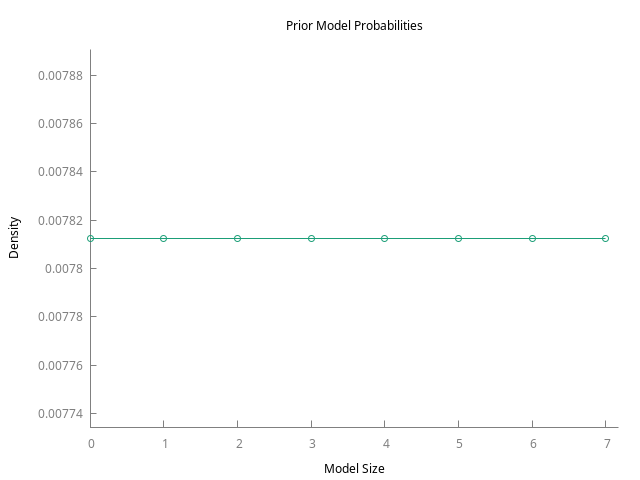
\includegraphics[width=1\textwidth]{PNG/ModelPriorDist_uniform}
		\caption{}
		\label{fig:model_priors:subfig:uniform}
	\end{subfigure}
	\begin{subfigure}[b]{0.24\textwidth}
		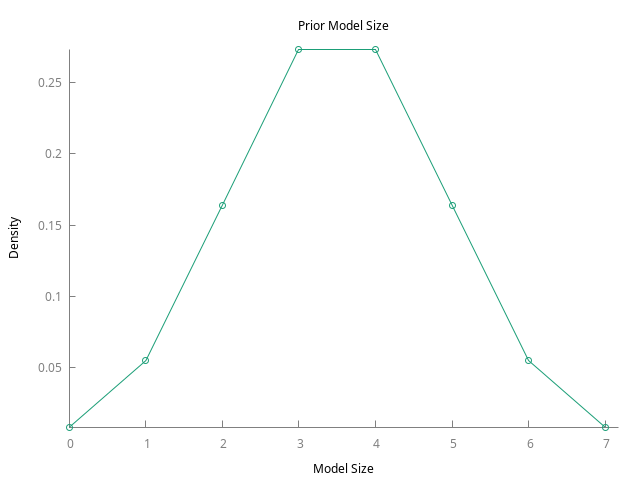
\includegraphics[width=1\textwidth]{PNG/ModelSizePriorDist_uniform}
		\caption{}
		\label{fig:model_priors:subfig:uniform-size}
	\end{subfigure}
	\begin{subfigure}[b]{0.24\textwidth}
		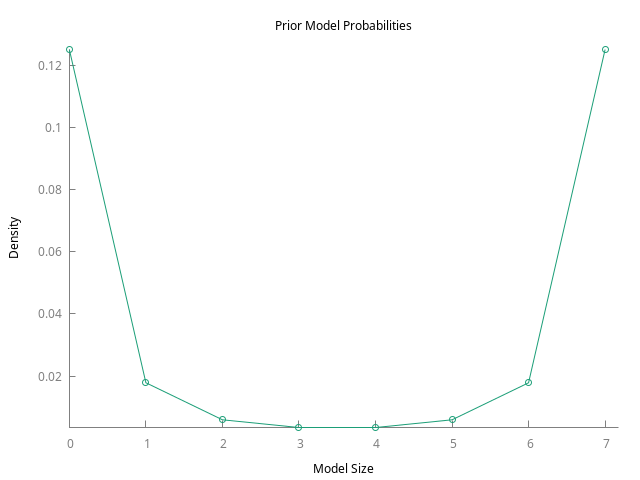
\includegraphics[width=1\textwidth]{PNG/ModelPriorDist_beta-binomial}
		\caption{}
		\label{fig:model_priors:subfig:beta-binomial}
	\end{subfigure}
	\begin{subfigure}[b]{0.24\textwidth}
		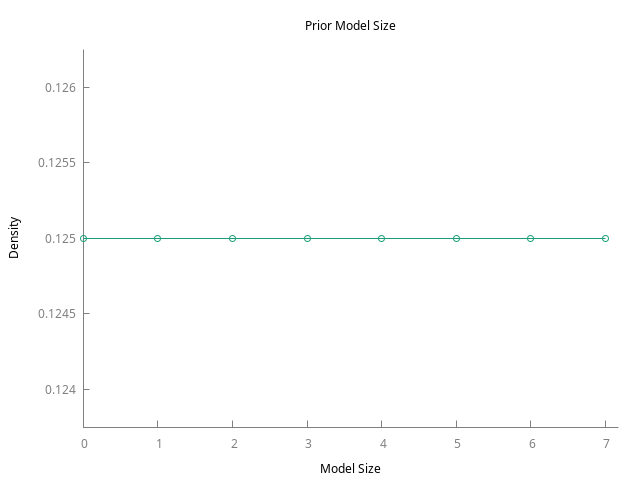
\includegraphics[width=1\textwidth]{PNG/ModelSizePriorDist_beta-binomial}
		\caption{}
		\label{fig:model_priors:subfig:beta-binomial-size}
	\end{subfigure}
	\caption{Prior model probabilities with associated prior
		model size for $K=7$ and $W^\star=\frac{K}{2}$,
		when model includes constant term}
\end{figure}

Sometimes, in a regression model, we do not include a constant
term \citep[see][]{KrolzigHendry-Computer_automation-2001,Kufel_jae_2020}.
This modelling strategy means that the model space is reduced
to $2^{K-1}$ possible combinations by excluding one specification
that consists of only a constant term, i.e., a model with no
explanatory variables. As a consequence, we should reflect
this in the \pkg{BACE} modeling by using a truncated prior
model size distribution.

From the definition of conditional probability, we can
define the density of a truncated random variable as
\cite[see][pp~864]{greene_econometric_a}:
\begin{equation}
	f\left(x | x > a\right) = \frac{f(x)}{\Prob(x > a)} .
\end{equation}
Because in our package, we assume that the user defines only
the expected model size $\E(W) = W^\star$, we have to rescale
the prior model size distribution so that it sums up to 1 and
has an expected value equal to $W^\star$. To do this, we have
to find the root of the following equation
\citep[see][]{Atwood1980,TripathiGuptaGurland-Estimation-1994}:
\begin{equation}
	\frac{\E(W)}{1-\Prob(W=0)} - W^\star = 0.
	\label{eq:solve_for_truncated_dist}
\end{equation}
We solve Equation~(\ref{eq:solve_for_truncated_dist})
numerically using \pkg{gretl}'s built-in \gretlcmd{fzero}
function. Note that for edge cases, i.e., when
$W^\star\approx 0$ or $W^\star\approx K$, the solution to
Equation~(\ref{eq:solve_for_truncated_dist}) may not exist.
Examples for $K=7$ are shown in
Figures~\ref{fig:model_priors:subfig:uniform-TR}-%
\ref{fig:model_priors:subfig:beta-binomial-size-TR}.

\begin{figure}[h!]
	\centering
	\begin{subfigure}[b]{0.24\textwidth}
		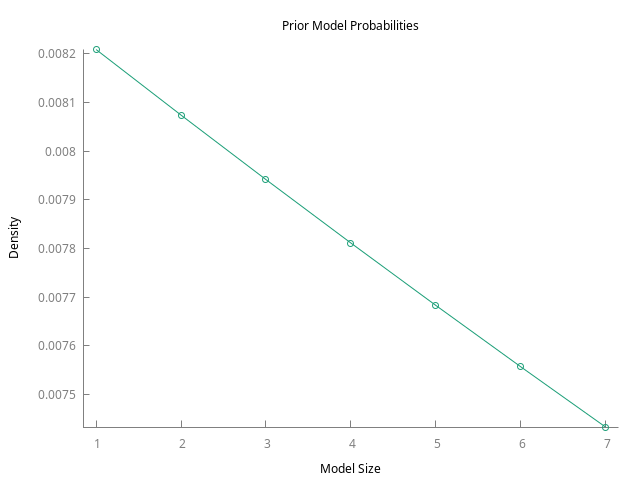
\includegraphics[width=1\textwidth]{PNG/ModelPriorDist_uniform-TR}
		\caption{}
		\label{fig:model_priors:subfig:uniform-TR}
	\end{subfigure}
	\begin{subfigure}[b]{0.24\textwidth}
		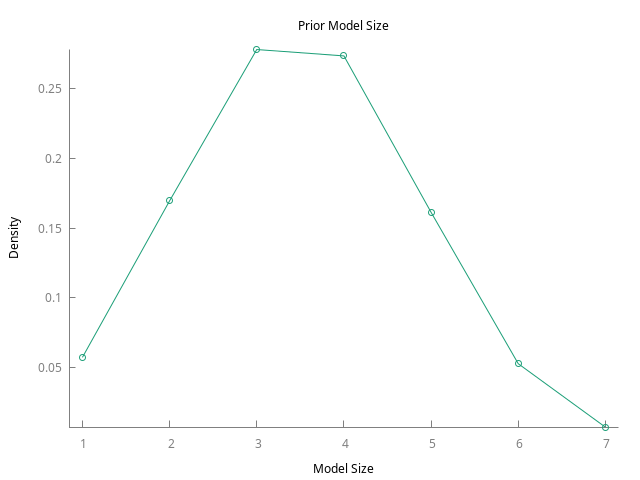
\includegraphics[width=1\textwidth]{PNG/ModelSizePriorDist_uniform-TR}
		\caption{}
		\label{fig:model_priors:subfig:uniform-size-TR}
	\end{subfigure}
	\begin{subfigure}[b]{0.24\textwidth}
		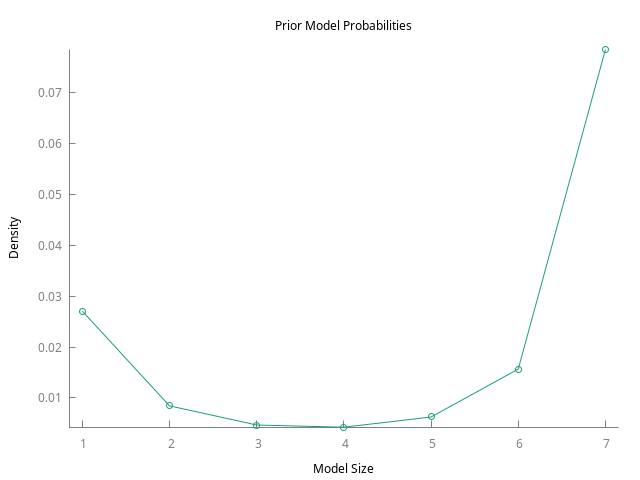
\includegraphics[width=1\textwidth]{PNG/ModelPriorDist_beta-binomial-TR}
		\caption{}
		\label{fig:model_priors:subfig:beta-binomial-TR}
	\end{subfigure}
	\begin{subfigure}[b]{0.24\textwidth}
		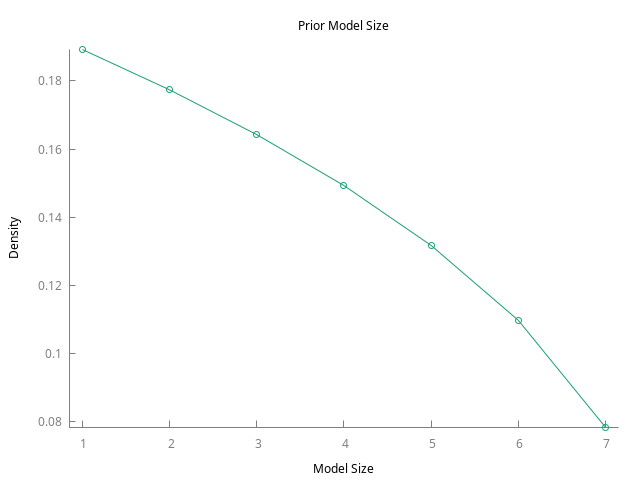
\includegraphics[width=1\textwidth]{PNG/ModelSizePriorDist_beta-binomial-TR}
		\caption{}
		\label{fig:model_priors:subfig:beta-binomial-size-TR}
	\end{subfigure}
	\caption{Prior model probabilities with associated prior
	model size for $K=7$ and $W^\star=\frac{K}{2}$,
		when model does not include a constant term}
\end{figure}

On the basis of Bayes' formula, the posterior probability
of any model $M_j$ can be computed as follows:
\begin{equation}
	\Prob(M_j|y) = \frac{\Prob(M_j)p\left( y \mid M_j\right)}
	{\sum_{r=1}^{2^K}\Prob(M_r)p\left( y \mid M_r\right)}
	\label{eq: model_avg}
\end{equation}
It is easy to see that Equation \ref{eq: model_avg} allows
us to calculate the probability for each model $M_r$ using
corresponding prior probabilities $\Prob\left( M_r\right)$ and
the density of the marginal distribution $p(y \mid M_j)$,
here approximated by expressions \ref{eq: BIC} -- \ref{eq: IBIC}.

Another useful characteristic popular in the model averaging
approach is the Posterior Inclusion Probability (PIP), which
is defined as the posterior probability that the independent
variable $x_i$ is relevant in explaining the dependent variable
(\cite{Leamer1978, mitchell_beauchamp_1988}). In our case, the
PIP is calculated using Monte Carlo integration, as the sum of
the posterior model probabilities for all models that include
the specific independent variable \citep{Forte_Garcia_Steel_2018}.

Although posterior characteristics are often of interest,
predicting future values of the dependent variable can be
valuable in many cases. With the \pkg{BACE} approach, we can
also perform predictive inference across the entire model space.
If we have the matrix $X_r^*$ containing explanatory variables
for each of the out-of-sample data points, we can use a
weighted average of the individual model forecasts to make
predictions about unobserved values of the dependent variable.

To determine the significance of determinants and the most
likely models across the model space, we utilize the \MCcube
sampling algorithm, which was originally developed by
\cite{madiganyork1995}. The \MCcube algorithm is one of the most
widely used MCMC algorithms in many statistical packages for
model averaging, for example:
\cite{LamnisosGriffinSteel2013,JSSv068i04,rafteryhoetingvolinskypainteryeung_bma,JSSv104i02}.
